\documentclass[12pt]{article}%
\usepackage{amsmath,amssymb,amsthm,amsfonts}
\usepackage{wasysym}
\usepackage{graphicx}
\usepackage[dvipsnames]{xcolor}
\usepackage{stackengine}
\def\stackalignment{l}
\usepackage[colorlinks]{hyperref}
\usepackage{tikz}
\usepackage[export]{adjustbox}

%\usepackage{geometry}
%\geometry{top = 0.9in}
\usepackage{appendix}

\usepackage{commands}

\newcounter{subfigure}

\renewcommand{\epsilon}{\varepsilon}
\renewcommand{\th}{\text{th}}
\newcommand{\sgn}{\operatorname{sgn}}

\renewcommand{\setminus}{\smallsetminus}

\newtheorem{thm}{Theorem}
\newtheorem{lemma}{Lemma}

\definecolor{red}{rgb}{0.8500, 0.3250, 0.0980}
\definecolor{green}{rgb}{0.4660, 0.6740, 0.1880}
\definecolor{yellow}{rgb}{0.9290, 0.6940, 0.1250}
\definecolor{blue}{rgb}{0, 0.4470, 0.7410}


\begin{document}

\title{Coding Project 2:  Parsing musical frequency signatures}

\author{Marvyn Bailly}
\date{February 10, 2023}

\maketitle


\begin{abstract}
In this paper, we begin with a brief explanation on musical notes and their associated frequencies. We continue to discuss elements of the mathematical theory behind the Gabor Transform and the Discrete Gabor Transform. Next we demonstrate how to apply numerical methods to create a spectrogram of a song. Using the spectrogram, we pick out frequencies of individual instruments and use a frequency filter to isolate their signal. We conclude by analyzing the isolated signals and discussing how the strengths and weaknesses of using the Discrete Gabor Transform. 
\end{abstract}


\section{Introduction}
\label{Sec: Intro}

Throughout each of our days, we encounter many different noises ranging from pleasant to harsh but almost all of these sounds have some form of meaning to us. We find the meaning by translating specific frequencies of the sound waves into patterns our brains understand. But what if many of these waves are layered on top of each other? In most cases, the collection of sound causes a cacophony but if applied correctly, can create beautiful musical harmonies. To allow for the creation of consistent and recognizable musical pieces across different instruments and cultures, the concept of assigning specific frequencies to musical notes has been widely accepted and used for centuries. For example, the frequency of middle C on a piano is approximately 261.63 Hz.. 


\bigskip
\bigskip

In this coding projecting, we will explore the application of the Gabor Transform on a song clip to isolate the frequencies of different instruments. We begin by explaining the mathematical theoretical background of the Gabor Transform  and the Discrete Gabor Transform, going into detail on the derivation and motivation of each transform. Next we will demonstrate the numerical methods of the Gabor Transform applied to a sound clip of a song. The Gabor Transform will allow us to create a spectrogram which can be studied to locate the specific frequencies of instruments throughout the clip. Using a similar filtering process, we can isolate the frequencies of the baseline and guitar. Finally we will present our result from the numerical methods section before concluding with the benefits and drawbacks of using this technique.  


\section{Theoretical Background}

In this section, we will explore the derivations and motivation of the Gabor Transform and the Discrete Gabor Transform. 


\subsection{The Gabor Transform}

While the Fourier Transform is a crucial step in signal analysis, it has many limitations. One of these limitations is that while the Fourier Transform gives a lot of detail on the frequency domain, it fails to provide crucial information on about the time domain. This phenomenon is known as the Heisenberg Uncertainty Principal which states an inverse relationship between the information in the time and the frequency domain. That is, the more know about one domain, means less is known about the other. Specifically in our case when studying music signals, it is important to know information about both domains. Thus we need to modify the Fourier Transform to give more detail on the time domain.

The Gabor Transform begins by modifying the Fourier kernel by adding the term $g(\tau - t)$ which gives
\[ 
    g_{t,w}(\tau) = e^{i \omega \tau}g(\tau - t),
\]
with the aim to localize both time and frequency. Adding this term to the Fourier Transform gives the Gabor Transform also known as the Short-Time Fourier Transform which is of the form
\[ 
    \mathcal{G}[f](t,\omega) = \tilde{f}_g(t,\omega) = \int_{-\infty}^{\infty}f(\tau) \bar{g}(\tau - t)e^{-i\omega \tau}d\tau.
\]
The new term acts as a time filter which is centered at $\tau$ with a width $a$. Thus we have to choose an appropriate width to retain enough information on both domains. For our case, we can assume that $g$ is real and symmetric which gives 
\[ 
    \mathcal{G}[f](t,\omega) = \tilde{f}_g(t,\omega) = \int_{-\infty}^{\infty}f(\tau) g(\tau - t)e^{-i\omega \tau}d\tau.
\]

\subsection{The Discrete Gabor Transform}
The Discrete Gabor Transform is a digital version of the Gabor Transform that is modified to a discrete representation of the time-frequency information of a signal. To discretize, we preform the transformation on a lattice of the time and frequency where the lattice is of the form
\begin{align*}
    \nu &= m\omega_0,\\
    \tau &= nt_0,
\end{align*}
where $m,n$ are integers and $\omega_0,t_0$ are constants that are greater than zero. Plugging this into the Gabor Transform makes $g_{t,\omega}$ become
\[ 
    g_{m,n}(t) = e^{i2\pi m\omega_0 t}g(t-nt_0),
\]
and thus the Discrete Gabor Transform is
\[ 
    \tilde{f}(m,n) = \int_{-\infty}^{\infty}f(t)g_{m,n}(t)dt,
\]
under the assume that $g$ is real and symmetric.


\section{Numerical Methods}

To demonstrate the power of Gabor and Discrete Gabor Transforms, we consider a short audio clip from a song. We will use MATLAB to preform the numerical methods. To begin, we set up the project by loading the clip into MATLAB with a sample rate of $44100$ samples per second and break it up into four smaller length windows which will be easier to work with. Next we find the length of each window in seconds ($L$) and the number of elements in each window ($n$). We continue to define the variable $t$ as vector representing the time in seconds relative to the start of each window, while the variable $\tau$ is a discretized vector of values that will be used for the Discrete Gabor Transform. Finally, The variable $k$ is a discretized vector of frequencies in the frequency domain, and $ks$ is the same as $k$ but shifted using the MATLAB's \verb+fftshift+ function. 

Now that we have set up the project, we first wish to use the Discrete Gabor Transform to create a spectrogram of the frequencies from the audio clip. We begin by looping over the discretized time vector $\tau$. For each iteration, we first create a Gabor Function with width $400$, multiple the Gabor Function with the desired window of audio, and apply a Fast Fourier Transform using MATLAB's \verb+fft+ function, saving the result in variable $Sgt$. Since we are iterating over the discretized time values, this is acting as a moving window filter over time. Next we find the max peak value of the frequency of $Sgt$ using MATLAB's \verb+max+ function. This allows us to create and apply a Gaussian Frequency Filter centered around the peak frequency to isolate the major effects. Finally we us MATLAB's \verb+fftshift+ to shift the output so that the zero-frequency component is in the center. Repeating this process for each window and plotting the result yields a spectrogram, as seen in Figure 1., for the audio clip. 

Finally we wanted to use the spectrogram to isolated the baseline and the guitar of the song respectfully. To do this, we studied the spectrogram (see \ref{Sec: Results} Results) to find the approximate range of frequencies corresponding to each instrument. After finding appropriate bounds for each instrument, we Fast Fourier Transformed the song into the frequency domain and set all frequencies outside of the determined threshold to zero. Applying the Inverse Fast Fourier Transform gave the signal clip for the isolated instrument.    

\begin{figure}
    \center
    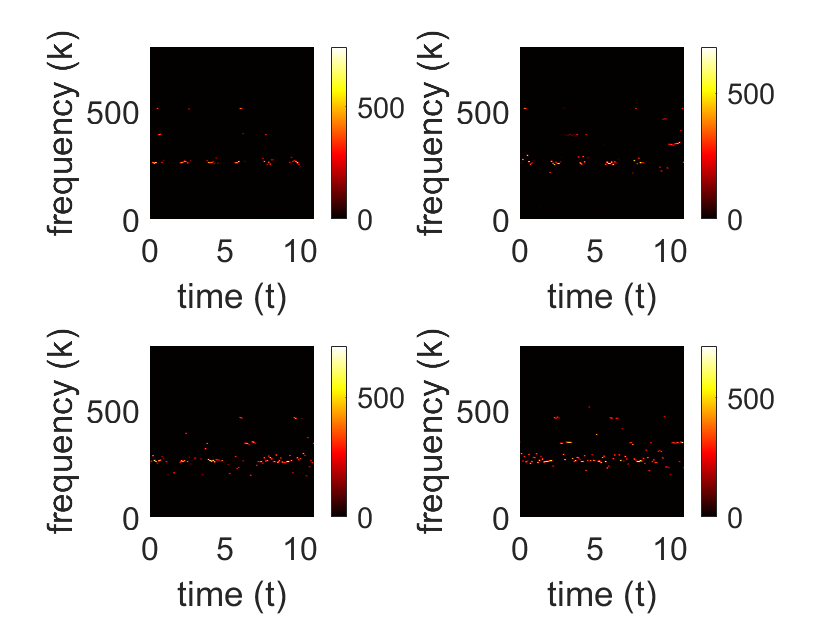
\includegraphics[width = 0.8\linewidth]{specto1.png}
    \caption{Spectrogram of Gabor Transformed audio clip in four windows.}
\end{figure}

\section{Results} \label{Sec: Results}

Applying the numerical methods described the previous section on the audio clip of a song, yields a spectrogram of the Gabor Transformed frequencies in time. Each window corresponds to a clip of the audio we split into four sections. The heat map shows consistent patterns of peak frequencies around $250$ which we believed to correspond to the baseline. We can to this conclusion in two ways. Firstly, we know that lower music notes, such as those heard in a baseline, correspond to low frequencies. And secondly that the baseline had a consistent rhythm that corresponded to the pattern at around $250$. Thus we choice a threshold of a minimum frequency of $60$ and an upper of $250$. To find the threshold for the guitar, we figured that the high pitches of a guitar instrument placed it higher on the spectrogram. Additionally, we listened to the original song for when the guitar started playing and found the corresponding patches on the Spectrogram. This lead us to believe that the highest patches on the spectrogram, around $500$, corresponded to the guitar. Thus we choice the threshold of a minimum frequency of $450$ and an upper of $550$. 

First we filtered the baseline using the threshold we found and the numerical method described above. The resulting signal corresponded to an approximate isolation of the baseline which allowed us to listen to just the baseline and plot its frequencies. Initially we experienced confusion since the resulting audio did not exhibit the baseline but rather a messy mix of the lower frequencies in the song. After changing the threshold a few times and having the same result, we figured out that it was a hardware issue rather than in the code. Testing the code with a different computer gave a fairly decent isolation of the baseline with some information lost and some noise coming in from the other instruments. Plotting the amplitude of the frequencies compared to the original clip as seen in Figure 2 revealed the amplitude of the baseline. We can see the consistent beat of the baseline and how it fits into the original piece. Towards the end of the time, the plot becomes less clear due to the complexity of the song increasing. 

Next we carried out a similar process to isolate the guitar in the song. Using the threshold we found (and someone else's computer to play the audio) the resulting audio clip had isolated the guitar. Once again there was some extra noise from the song but the filter mostly succeeded in isolating the guitar. Plotting the guitar amplitude compared to the original, as seen in Figure 3., showed that at first the guitar was not very obvious in the song but continued to become a major part of the song. Since we used a sticker threshold for the guitar, the ending section of the plot seems more reasonable than in Figure 2. despite the complexity of the song.  

\begin{figure}
    \center
    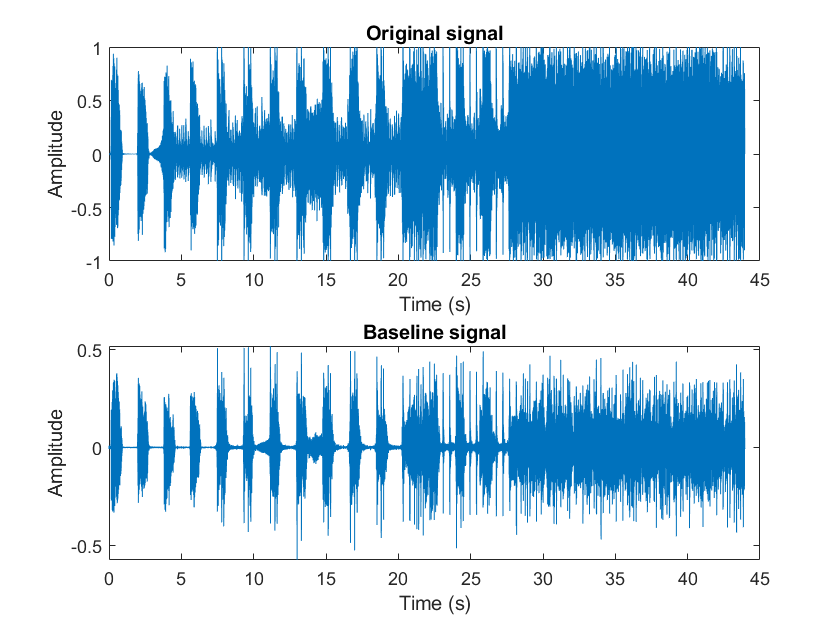
\includegraphics[width = 0.6\linewidth]{baseline.png}
    \caption{Amplitude of the baseline signal over time compared to the original audio signal.}
\end{figure}
    
\begin{figure}
    \center
    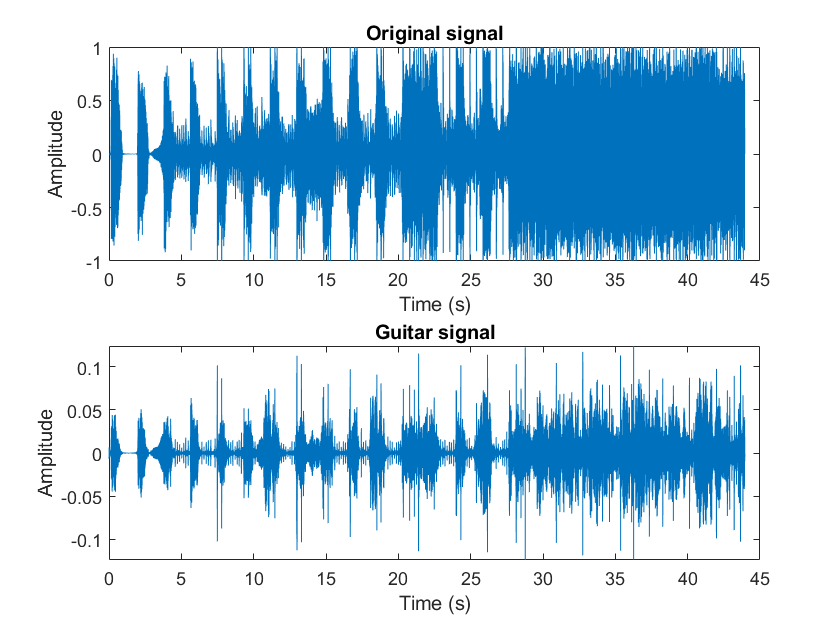
\includegraphics[width = 0.6\linewidth]{guitarline.png}
    \caption{Amplitude of the guitar signal over time compared to the original audio signal.}
\end{figure}

\section{Conclusion}\label{Sec: Conclusion}

In this coding project, we briefly gave background information on how music is understood through different levels of frequencies. Next we discussed the theoretical background of the Gabor Transform and the Discrete Gabor Transform before demonstrating how to isolate and reconstruct various instrument types present in the song clip. The process involved two main steps, starting with the creation of a spectrogram using the Discrete Gabor Transform. Next we isolated the baseline from the sound clip using a frequency filter, followed by the isolation of the guitar. The sound clip used in the project has the advantage of having the instruments introduced one at a time, making it easier to isolate their frequency signatures.

Throughout the project we learned how to numerically apply the mathematical theory and techniques discussed in Section 2 in MATLAB. We saw the power of creating a spectrogram using the Discrete Gabor Transform to pick out the frequency ranges of various instruments by applying a frequencies filter using our estimate thresholds. These thresholds proved to be reasonable accurate when listening to the audio. Some of the drawbacks in using the spectrogram is that the was the use of guess work to determine the thresholds of the instruments. We also loose information about both domains when using the Gabor Transform and thus it might be better to use a different type of transformation for music. It would be interesting to come up with a way to automate the process so that any audio clip could be filtered using our code. Additionally, a different filtering methods could be applied to reduce the amount of extra noise in the final clips.  



\section*{Acknowledgment}

A special thanks to Alex Johnson and Charbel Younes who I worked with throughout this coding project. 

\end{document}
